\documentclass[journal]{IEEEtran}

\usepackage[utf8]{inputenc}
\usepackage[T1]{fontenc}
\usepackage[spanish,english]{babel}
\addto\captionsenglish{\renewcommand{\abstractname}{Abstract}}
\usepackage{graphicx}
\usepackage{amsmath}
\usepackage{array}
\usepackage{float}
\usepackage{url}
\usepackage{booktabs}
\usepackage{multirow}
\usepackage{hyperref}
\usepackage{subcaption}
\graphicspath{{images/}{anexos/github-controles/}}
\newcommand{\evidenceimage}[2]{%
  \IfFileExists{images/#1}{\includegraphics[width=0.96\columnwidth]{#1}}{%
    \fbox{\parbox[c][3.0cm][c]{0.90\columnwidth}{\centering
    \textbf{Evidence image pending}\\[2pt]\texttt{#1}\\[2pt]
    Copy this file from the GitHub evidence folder into the \texttt{images/} directory.}}}%
  \caption{#2}%
}

\title{Seguridad de Aplicaciones\\
\large \textit{SAST, DAST y Pentesting autorizado}\\
\normalsize De GitHub a un pipeline de seguridad}

\author{Brayan Loaiza Leal,
Juan Sebastián Guayazán Clavijo
\thanks{Entrega final}
\thanks{Fundamentos de Seguridad de la Información}
\thanks{Ingeniería de Sistemas}
\thanks{Escuela Colombiana de Ingeniería Julio Garavito}
\thanks{2026-2, Tercer Tercio}}

\markboth{Laboratorio 05 --- Seguridad en el ciclo de desarrollo}{Seguridad de Aplicaciones}

\begin{document}
\selectlanguage{spanish}
\maketitle

\begin{otherlanguage}{english}
\begin{abstract}
This laboratory evaluates the security of the \textit{CrowdStrike Falcon Alert Simulator} through Static Application Security Testing (SAST), secret detection, Software Composition Analysis (SCA), and passive Dynamic Application Security Testing (DAST). The report describes the project baseline, GitHub security configuration, and the results obtained with Semgrep, Gitleaks, Dependabot, and OWASP ZAP. A controlled validation of Log Injection (CWE-117) confirmed that an attacker-controlled line break could create forged log entries. The remediation was integrated through Pull Request (PR) \#8 and supported by regression evidence. The report also documents the Nginx Host header issue (F-16), corrected in PR \#9, which remains pending integration, as well as the dependency update proposed by Dependabot and the limitations of the tests performed.
\end{abstract}
\begin{IEEEkeywords}
Application security, DevSecOps, SAST, DAST, SCA, GitHub Actions, OWASP ZAP.
\end{IEEEkeywords}
\end{otherlanguage}

\section{Introducción}
La seguridad debe incorporarse durante el desarrollo de software y verificarse mediante controles que produzcan evidencia. En este laboratorio se evaluó el proyecto del equipo, se analizaron resultados de seguridad, se validó un riesgo técnico en un entorno controlado y se documentaron las correcciones mediante Pull Requests y pruebas de regresión.

\section{Alcance y línea base}
\subsection{Proyecto y entorno}
\begin{table}[H]
\centering
\caption{Identificación y línea base del proyecto}
\label{tab:baseline}
\begin{tabular}{|p{0.34\columnwidth}|p{0.55\columnwidth}|}\hline
\textbf{Campo} & \textbf{Dato} \\ \hline
Proyecto & CrowdStrike Falcon Alert Simulator \\ \hline
Repositorio & \url{https://github.com/BrayanLoaiza-JuanGuayazan-FDSI/Lab3-FDSI} \\ \hline
Responsables & Brayan Loaiza Leal y Juan Sebastián Guayazán Clavijo \\ \hline
Tecnología & Python 3.12, Flask 3.1.3, Werkzeug 3.1.9, Nginx y frontend HTML/JavaScript \\ \hline
APIs & Alerts API (5000) y Actions API (5001), publicadas mediante Nginx \\ \hline
Autenticación & Encabezado \texttt{X-API-Key}; excepción para \texttt{/health} \\ \hline
Rama del laboratorio & \texttt{security/lab-fsi} \\ \hline
Commit de línea base & \texttt{6440081} \\ \hline
Entorno de validación & Docker local aislado, servicios en loopback y datos ficticios \\ \hline
\end{tabular}
\end{table}

La arquitectura evaluada contiene un frontend estático servido por Nginx y dos APIs Flask. Nginx recibe las solicitudes y las dirige a Alerts API y Actions API. Las APIs utilizan el encabezado \texttt{X-API-Key} en sus rutas, excepto \texttt{/health}. El repositorio y los servicios son propios del equipo.

Las pruebas se limitaron al repositorio y al entorno local controlado con datos ficticios. No se evaluaron sistemas de terceros ni producción, ni se realizaron acciones destructivas. Para DAST se utilizó la alternativa local con Docker indicada en el enunciado, dado que no se dispuso de un staging HTTPS.

\section{Controles automatizados y resultados}
\subsection{SAST y CodeQL}
Semgrep se ejecutó en GitHub Actions mediante \texttt{.github/workflows/security.yml}. La secuencia de resultados fue de 15 en la línea base, 2 después de excluir las copias históricas F-17 y de la primera remediación, y 0 tras corregir F-16 en Nginx. Las dos coincidencias restantes correspondían a \texttt{proxy\_set\_header Host \$host;} en los dos proxies. El cambio a \texttt{\$proxy\_host} eliminó las coincidencias en el reescaneo.

CodeQL Default setup quedó habilitado para GitHub Actions, JavaScript/TypeScript y Python. La captura de configuración y análisis corresponde a una revisión anterior a la corrección F-15; se presenta como evidencia de configuración, no como garantía de ausencia de vulnerabilidades. El PR \#10 contiene diez capturas de configuración, lenguajes analizados y alertas de Code Scanning, Dependabot y Secret Scanning; se consultan en \href{https://github.com/BrayanLoaiza-JuanGuayazan-FDSI/Lab3-FDSI/tree/docs/github-security-controls/anexos/github-controles}{la carpeta de evidencias de GitHub}.

\begin{figure}[H]
\centering
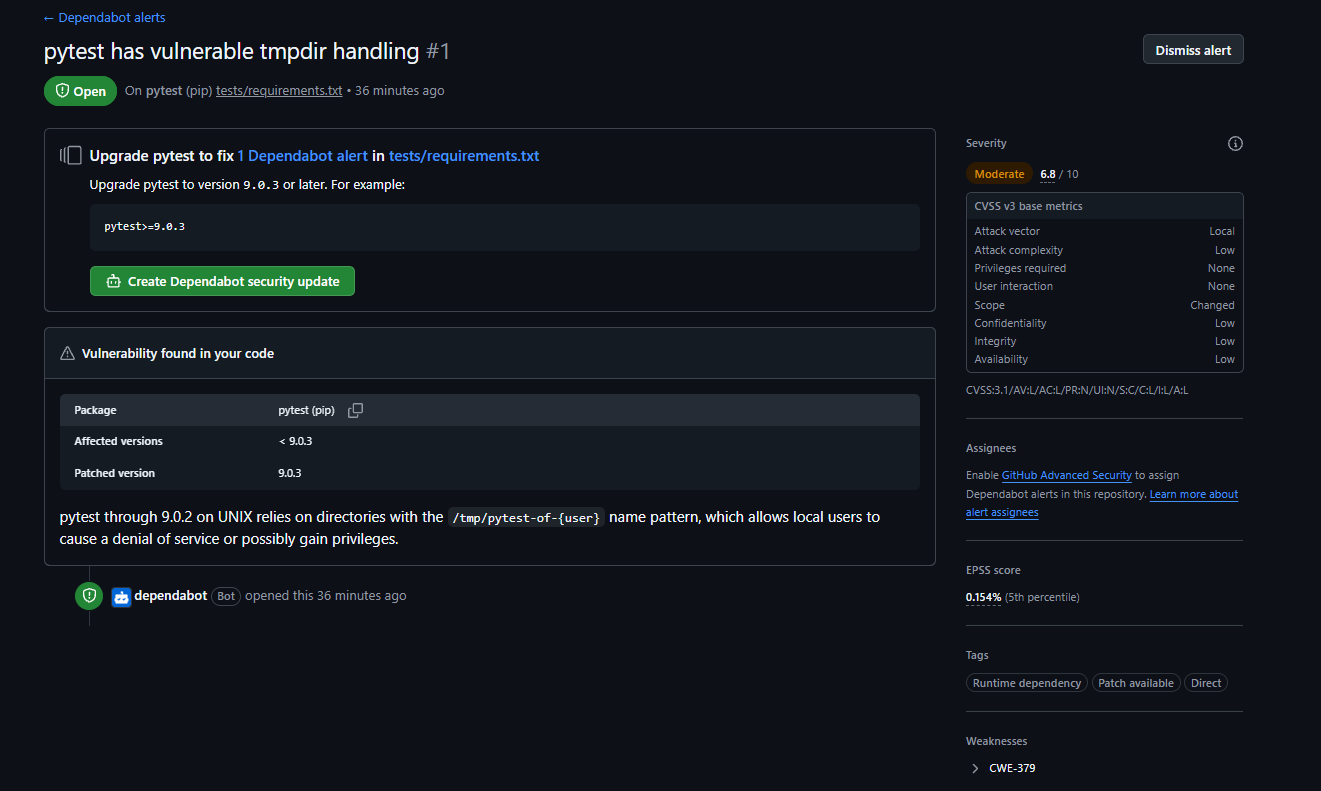
\includegraphics[width=0.96\columnwidth]{dependabot-alerta-pytest.png}
\caption{Alerta Dependabot de pytest: versión corregida 9.0.3 y severidad moderada.}
\label{fig:pytest-alert}
\end{figure}

\subsection{Análisis dinámico (DAST)}
El 10 de noviembre de 2026, entre las 23:48 y las 23:50 (hora de Colombia), se ejecutó OWASP ZAP 2.17.0 mediante \texttt{zap-baseline.py} en modo pasivo. Se evaluó \texttt{main}, commit \texttt{27a871a}, en una red Docker aislada denominada \texttt{lab5-dast}, con datos ficticios. Se analizaron el frontend, Alerts API y Actions API. Para las APIs se configuró una credencial de staging mediante la regla \texttt{replacer}; los reportes registran respuestas 2xx y 3xx y no muestran 401.

\begin{table}[H]
\centering
\caption{Resultados de OWASP ZAP Baseline}
\label{tab:zap}
\begin{tabular}{|l|c|c|c|c|}\hline
\textbf{Objetivo} & \textbf{High} & \textbf{Medium} & \textbf{Low} & \textbf{Info.} \\ \hline
Frontend & 0 & 0 & 4 & 2 \\ \hline
Alerts API & 0 & 0 & 5 & 2 \\ \hline
Actions API & 0 & 0 & 4 & 2 \\ \hline
\end{tabular}
\end{table}

Los tres análisis registraron cero alertas High y Medium y \texttt{FAIL-NEW=0}. Los resultados relevantes fueron: (D-01) respuestas de las APIs sin \texttt{Cache-Control}, clasificado como relevante de prioridad baja; (D-02) ausencia de Permissions Policy, oportunidad de endurecimiento de prioridad baja; y (D-03) alertas de cabeceras Cross-Origin, de baja relevancia dado que el sitio no carga recursos de otros orígenes y cuenta con CSP y \texttt{frame-ancestors 'none'}. ZAP también reportó D-04, Private IP Disclosure, clasificado como falso positivo porque \texttt{192.168.1.105} corresponde al indicador ficticio ALT-002 del simulador; y D-05, Modern Web Application, que es informativo y no representa por sí mismo un riesgo.

\begin{figure*}[t]
\centering
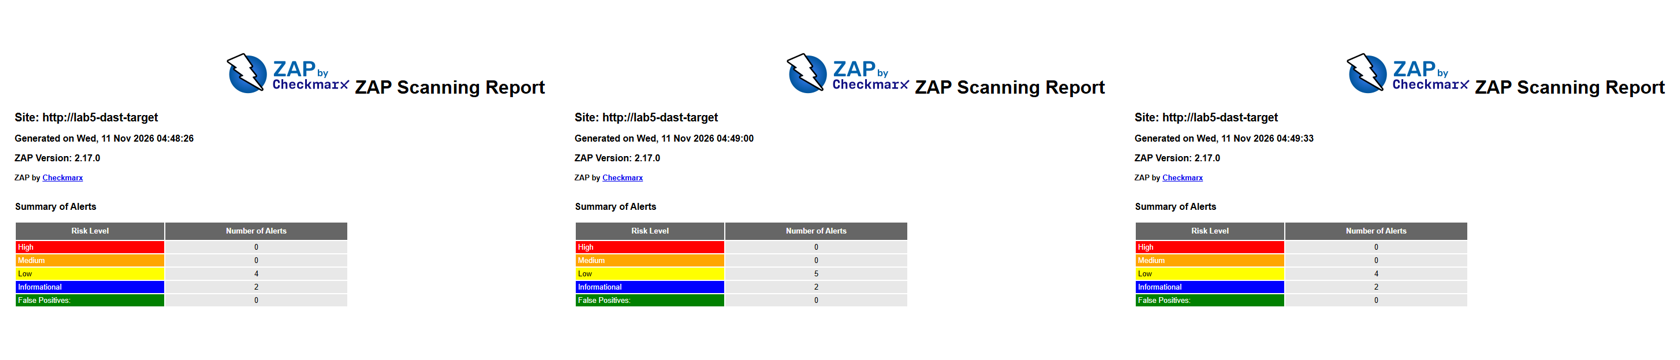
\includegraphics[width=0.96\textwidth]{dast-resumen-tres-objetivos.png}
\caption{Resumen de los tres análisis pasivos de OWASP ZAP.}
\label{fig:zap-summary}
\end{figure*}

Los reportes HTML, JSON, salidas de terminal y capturas de cada análisis se conservan en \texttt{anexos/dast/}. El análisis fue local y por HTTP; no evaluó TLS y no incluye el cambio de Nginx propuesto en el PR \#9.

\begin{figure*}[t]
\centering
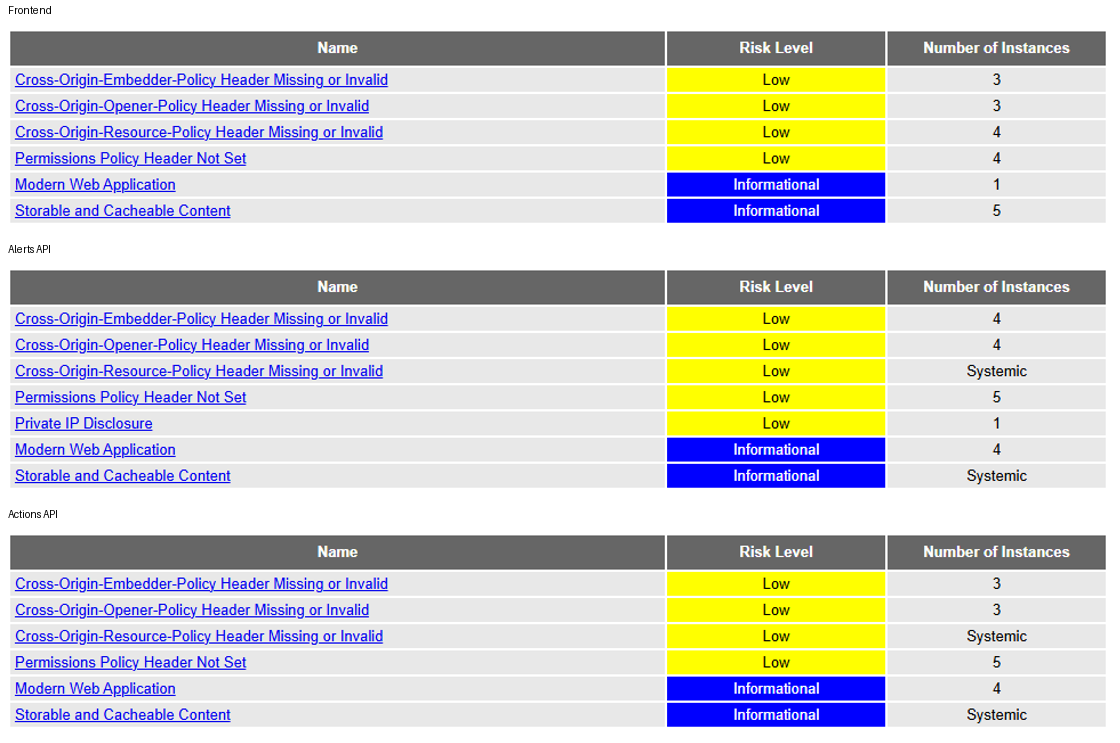
\includegraphics[width=0.96\textwidth]{dast-alertas-detalle.png}
\caption{Detalle de alertas pasivas reportadas por ZAP para frontend, Alerts API y Actions API.}
\label{fig:zap-alerts}
\end{figure*}

\section{Análisis y priorización de hallazgos}
La presentación de clase solicita analizar al menos tres hallazgos o resultados relevantes, incluidos falsos positivos justificados. La Tabla~\ref{tab:findings} resume los resultados del Laboratorio 5; no incorpora hallazgos del Laboratorio 3 que no formen parte de esta evaluación.

\begin{table}[H]
\centering
\caption{Matriz de hallazgos y decisiones}
\label{tab:findings}
\scriptsize
\setlength{\tabcolsep}{2pt}
\renewcommand{\arraystretch}{1.15}
\resizebox{\columnwidth}{!}{%
\begin{tabular}{|p{0.07\columnwidth}|p{0.19\columnwidth}|p{0.12\columnwidth}|p{0.28\columnwidth}|p{0.25\columnwidth}|}\hline
\textbf{ID} & \textbf{Resultado} & \textbf{Severidad} & \textbf{Evidencia} & \textbf{Decisión / estado} \\ \hline
F-15 & Log Injection (CWE-117) & Media & Validación manual con \texttt{\%0a}; antes se generaban líneas falsas y después no & Corregido e integrado en PR \#8 \\ \hline
F-16 & Encabezado Host en Nginx (CWE-290) & Baja & Dos coincidencias Semgrep; 0 tras el cambio & Corregido en rama del PR \#9; PR abierto \\ \hline
SCA-01 & pytest anterior a 9.0.3 (CWE-379) & Moderada & Alerta Dependabot en \texttt{tests/requirements.txt} & PR \#11 abierto; actualización pendiente \\ \hline
D-01 & API sin \texttt{Cache-Control} (CWE-524) & Info. / baja & ZAP pasivo y respuesta HTTP & Riesgo de caché; sin corrección registrada \\ \hline
D-04 & Private IP Disclosure (CWE-497) & Falso positivo & IP ficticia \texttt{192.168.1.105}, ALT-002 & No corresponde a infraestructura \\ \hline
F-18 & Coincidencia Gitleaks & Falso positivo & Valor deliberadamente inválido en prueba & Documentado; ejecución posterior sin resultados en el rango \\ \hline
F-17 & Coincidencias Semgrep históricas & Falso positivo & Cuatro coincidencias en archivos de evidencia no desplegados & Excluidas con \texttt{.semgrepignore} \\ \hline
\end{tabular}}
\end{table}

\section{Validación controlada y remediación}
Se validó F-15 (Log Injection, CWE-117) en Docker local, con datos ficticios y pasando por Nginx. La hipótesis era que un salto de línea codificado en la ruta podía generar una entrada falsa en \texttt{alerts.log}. Antes de la corrección, una petición produjo dos líneas, una de ellas con apariencia de evento \texttt{CRITICAL} falso. Después de la corrección, la secuencia quedó registrada como \texttt{\textbackslash n} literal y no se generaron líneas falsas. En ambos casos la solicitud respondió HTTP 404; el resultado relevante fue el contenido del registro.

La corrección de F-15 neutraliza CR/LF antes de escribir valores controlados por el usuario en los logs. En Actions API, los campos \texttt{analyst} y \texttt{alert\_id} se validan como cadenas antes de guardar la acción; los tipos no válidos se rechazan con HTTP 400. La corrección se integró en \texttt{main} mediante el PR \#8.

\begin{table}[H]
\centering
\caption{Evidencia antes y después de F-15}
\label{tab:f15}
\begin{tabular}{|p{0.25\columnwidth}|p{0.63\columnwidth}|}\hline
\textbf{Momento} & \textbf{Resultado observado} \\ \hline
Antes, commit \texttt{6440081} & Dos líneas con apariencia de evento; la entrada controlada podía contaminar el log. \\ \hline
Después, \texttt{main} \texttt{27a871a} & Una sola línea con \texttt{\textbackslash n} literal; cero líneas de evento falso. \\ \hline
\end{tabular}
\end{table}

\textbf{PR de F-15:} \href{https://github.com/BrayanLoaiza-JuanGuayazan-FDSI/Lab3-FDSI/pull/8}{Pull Request \#8}. La validación manual completa está en \texttt{anexos/validacion-f15.txt}.

\begin{figure}[H]
\centering
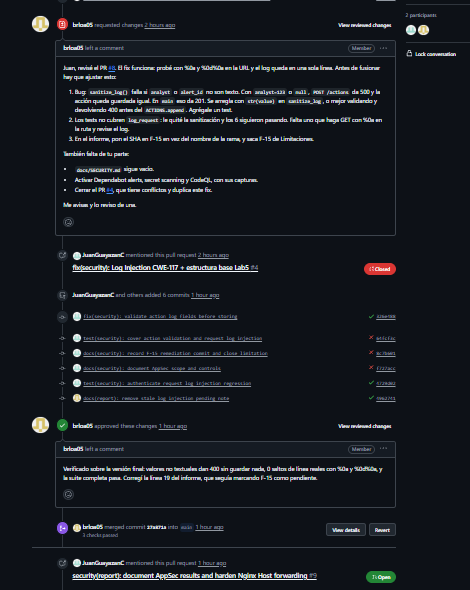
\includegraphics[width=0.65\columnwidth]{pr8-merge-crop.png}
\caption{Historial del PR \#8: revisión y fusión de la corrección F-15.}
\label{fig:pr8}
\end{figure}

F-17 correspondió a cuatro coincidencias de Semgrep en copias históricas de archivos de evidencia que no se despliegan. Se excluyeron mediante \texttt{.semgrepignore}; no se modificaron los archivos históricos.

F-16 se corrigió preventivamente en la configuración de Nginx: las dos directivas \texttt{proxy\_set\_header Host} cambiaron de \texttt{\$host} a \texttt{\$proxy\_host}. La validación en Docker confirmó que un Host falso llega a la API como \texttt{127.0.0.1:5000} y que las APIs, la autenticación y el dashboard continúan funcionando. Semgrep pasó de 2 coincidencias a 0 después del cambio. El PR \#9 está abierto y pendiente de aprobación e integración.

\textbf{PR de F-16:} \href{https://github.com/BrayanLoaiza-JuanGuayazan-FDSI/Lab3-FDSI/pull/9}{Pull Request \#9}.

\subsection{Reejecución de controles}
La ejecución \#28 del workflow de seguridad terminó con estado \texttt{success}: las pruebas de regresión, Semgrep y Gitleaks finalizaron correctamente. El artefacto Semgrep reportó 0 resultados y 0 errores en 27 rutas; Gitleaks reportó 0 resultados en el intervalo \texttt{HEAD\textasciitilde1..HEAD}. Los pasos de Semgrep y Gitleaks permiten continuar el workflow aun cuando existan resultados, por lo que el estado verde no sustituye la revisión de sus artefactos.

\textbf{Ejecución del workflow \#28:} \href{https://github.com/BrayanLoaiza-JuanGuayazan-FDSI/Lab3-FDSI/actions/runs/42956688617}{ver ejecución y jobs}.\\
\textbf{Workflow YAML:} \href{https://github.com/BrayanLoaiza-JuanGuayazan-FDSI/Lab3-FDSI/blob/main/.github/workflows/security.yml}{security.yml}.\\
\textbf{PR de controles y capturas:} \href{https://github.com/BrayanLoaiza-JuanGuayazan-FDSI/Lab3-FDSI/pull/10}{Pull Request \#10}.\\
\textbf{PR de SCA:} \href{https://github.com/BrayanLoaiza-JuanGuayazan-FDSI/Lab3-FDSI/pull/11}{Pull Request \#11}.\\
\textbf{Rama del laboratorio:} \href{https://github.com/BrayanLoaiza-JuanGuayazan-FDSI/Lab3-FDSI/tree/security/lab-fsi}{security/lab-fsi}.\\
\textbf{Documentación solicitada:} \href{https://github.com/BrayanLoaiza-JuanGuayazan-FDSI/Lab3-FDSI/blob/docs/github-security-controls/docs/SECURITY.md}{SECURITY.md} y \href{https://github.com/BrayanLoaiza-JuanGuayazan-FDSI/Lab3-FDSI/blob/docs/github-security-controls/docs/REPORTE_HALLAZGOS.md}{REPORTE\_HALLAZGOS.md}.

\begin{figure}[H]
\centering
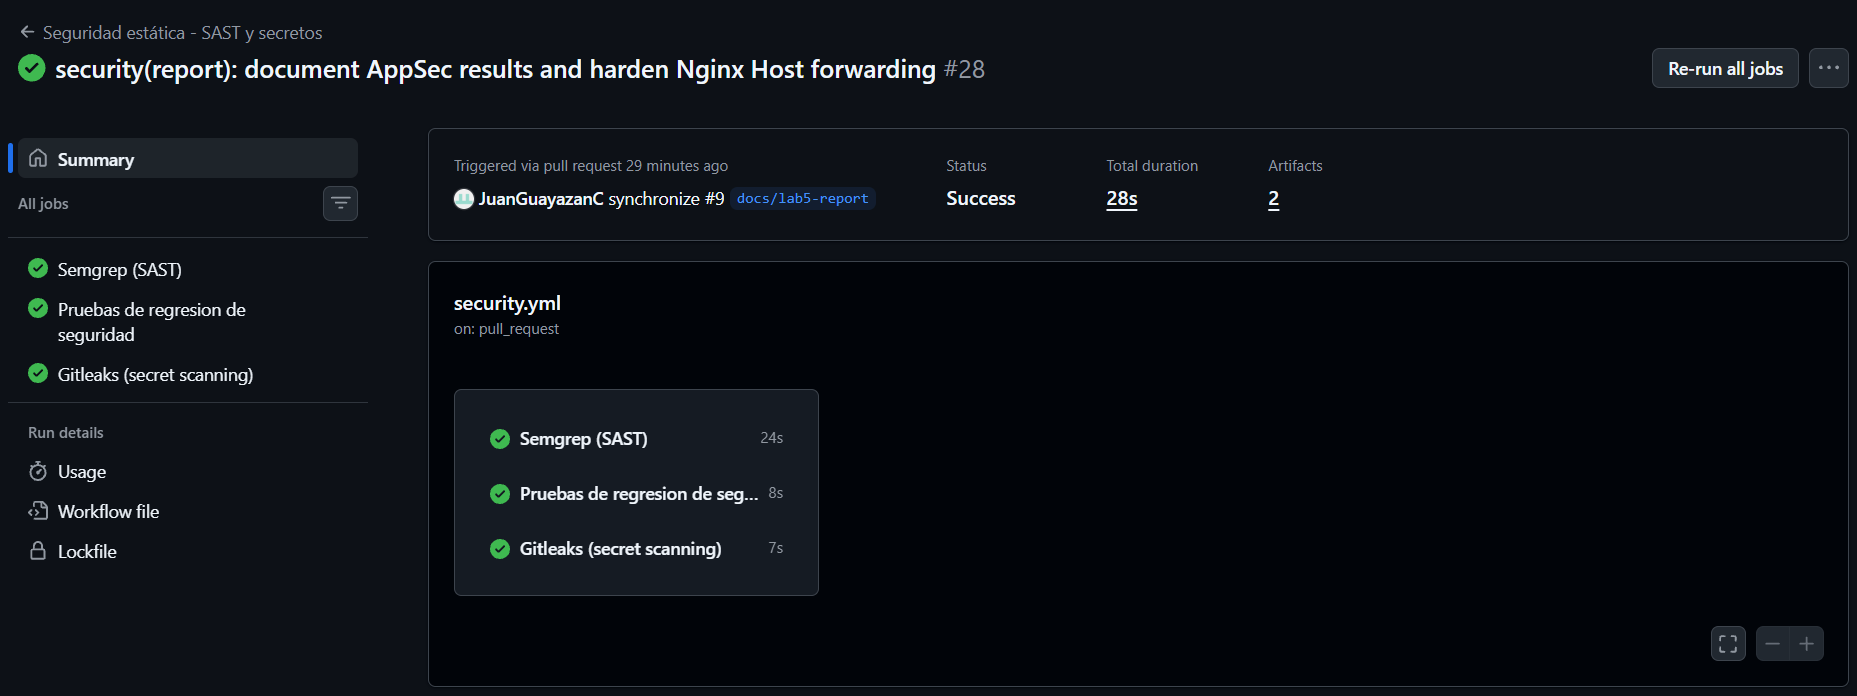
\includegraphics[width=0.96\columnwidth]{pipeline-resumen.png}
\caption{Ejecución \#28: los jobs Semgrep, pruebas de regresión y Gitleaks finalizaron correctamente.}
\label{fig:pipeline}
\end{figure}

\section{Resultados, limitaciones y entregables}
Los controles integrados y sus evidencias se resumen así:
\begin{itemize}
\item SAST y detección de secretos: workflow de GitHub Actions ejecutado; artefactos Semgrep y Gitleaks disponibles.
\item SCA: Dependabot alerts y actualizaciones configuradas; alerta de pytest registrada mediante PR \#11.
\item DAST: tres análisis OWASP ZAP Baseline pasivos, con reportes y capturas; se documentó la alternativa local con Docker.
\item Remediación: F-15 integrado mediante PR \#8 y prueba de regresión; F-16 corregido en PR \#9, aún abierto.
\end{itemize}

La demostración solicitada en el enunciado tiene una duración de cinco minutos; la presentación de clase solicita además un video de máximo tres minutos.

El DAST se ejecutó en HTTP local y no evaluó TLS. Sus resultados son pasivos y no demuestran ausencia de vulnerabilidades. El análisis se hizo sobre un commit de \texttt{main} anterior al cambio de Nginx del PR \#9. Gitleaks cubrió el intervalo de commits indicado, no todo el historial. CodeQL fue capturado antes de la corrección F-15. La actualización de pytest del PR \#11 todavía requiere integración y reejecución de pruebas.

\section{Conclusiones}
Se incorporaron controles SAST, detección de secretos, SCA y DAST pasivo al proceso de evaluación del proyecto. La validación controlada confirmó el riesgo de Log Injection y su corrección quedó integrada mediante el PR \#8, con evidencia antes y después. La corrección de F-16 eliminó las coincidencias de Semgrep en Nginx, pero el PR \#9 continúa pendiente de integración. Dependabot identificó una actualización de pytest que permanece en revisión. Los resultados se interpretan dentro del alcance de cada herramienta y de las limitaciones documentadas.



\end{document}